\section{Fragment-mixed continuation}
\label{sec:method}
\subsection{Task and notation}
Let $X=(x_1,\ldots,x_T)$ be the prepared mouth-image sequence of a source clip,
with transcript $y$. A visual encoder $f_\theta$ produces a sequence
$H=f_\theta(X)$, and CTC and attention heads define the recognition objectives.
The models used here preserve the temporal frame count through the encoder,
allowing a frame interval to index the corresponding encoded sequence.
At assessment, the desired output is the complete transcript
\begin{equation}
    \hat y = D_\alpha\bigl(f_\theta(X)\bigr),
    \label{eq:inference}
\end{equation}
where $D_\alpha$ is the selected decoder. No target interval, reference transcript,
word timestamp or crop decision is supplied during this inference.

For training only, let $I=[a,b)$ denote a fragment of $L=50$ frames, or two seconds
at 25 frames per second. The available word timings define its label as
\begin{equation}
 y_I = \operatorname{concat}\{w_k:
        e_k>a/25\ \text{and}\ s_k<b/25\},
 \label{eq:overlap}
\end{equation}
for positive-duration words with start and end times $(s_k,e_k)$.
Zero-duration entries are included only when their timestamp lies in the half-open
interval. The rule is based on overlap, not on whether the word is fully visible.
For example, a word ending just inside the fragment can be included even if most
of its articulation lies before $a$. Crop locations are drawn from precomputed
eligible starts, using the clip identifier, presentation index and random seed.
For a clip of $T$ frames, starts are enumerated at one-frame spacing from 16
through $T-66$ inclusive, retaining nonempty labels with a feasible CTC path.
A deterministic hash of the seed, clip identifier and presentation index selects
one retained start. This supplies 16 frames on either side for the paired context
control, even when FM itself uses only the core.

\subsection{Full-clip and fragment-mixed supervision}
Full-clip continuation (FC; experiment T0) minimizes the recognizer's existing
hybrid loss on each complete source clip:
\begin{equation}
 \mathcal L_{\rm ASR}(H,y)
 = 0.1\,\mathcal L_{\ctc}(H,y)
   +0.9\,\mathcal L_{\att}(H,y).
 \label{eq:asr}
\end{equation}
Fragment-mixed continuation (FM; T1) alternates full and fragment presentations:
\begin{equation}
 \mathcal L_{\rm FM}^{(j)} =
 \begin{cases}
  \mathcal L_{\rm ASR}(f_\theta(X),y), & j\text{ even},\\
  \mathcal L_{\rm ASR}(f_\theta(X_I),y_I), & j\text{ odd}.
 \end{cases}
 \label{eq:mix}
\end{equation}
Here $j$ indexes individual training presentations before gradient accumulation.
The same source clips occur in the same order for FC and FM within a seed.
Consequently, FM does not add previously unseen videos: it changes which part of
an already selected video is presented. At 6,000 optimizer updates with eight
presentations per update, each run contains 48,000 presentations. FM divides these
equally between complete clips and fragments.

The architecture is unchanged. The visual encoder and both recognition heads are
updated, while batch-normalization running statistics remain fixed. The native
loss reductions are retained: CTC is summed over the example and the attention
criterion aggregates valid token positions, with batch-size reduction rather than
explicit token-length normalization. Thus, matching updates does not match frames,
tokens or gradient magnitudes. We measure the first two directly in
Section~\ref{sec:exposure}; no proportional relationship between token count and
the final optimizer update is assumed.

\begin{figure}[tbp]
 \centering
 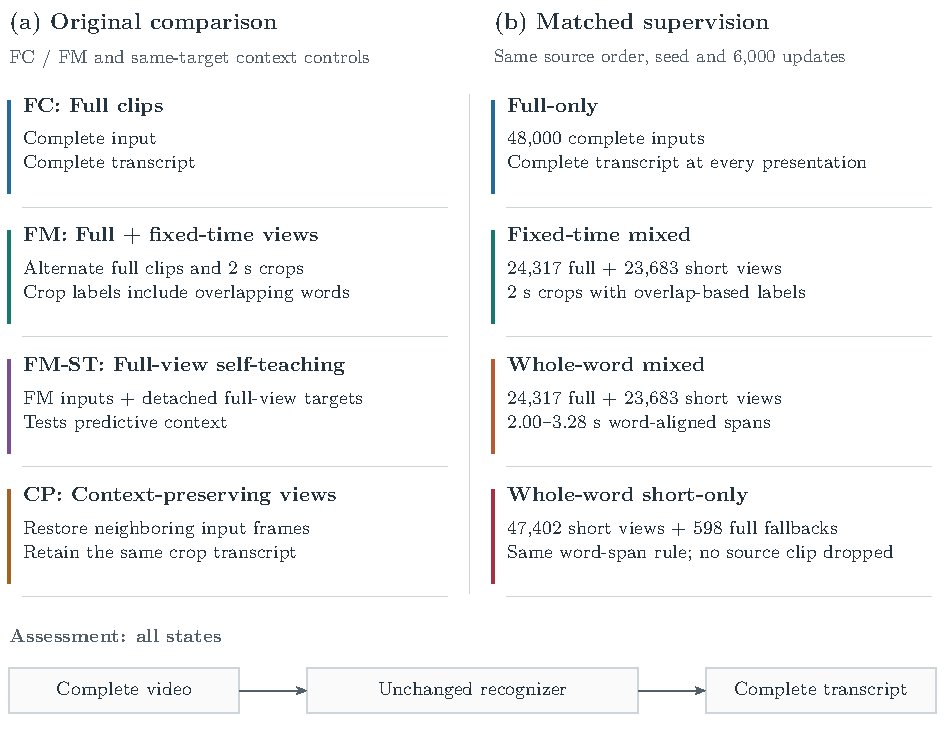
\includegraphics[width=\linewidth]{training_design.pdf}
 \caption{Training interventions with unchanged whole-utterance inference.
 (a) The original comparison tests full-clip continuation (FC), fragment mixing
 (FM), full-view self-teaching (FM-ST/T2), and restored visual context (CP/T4).
 (b) The matched comparison includes full-only, fixed-time mixed, whole-word
 mixed and whole-word short-only supervision. The mixed states share fallback
 positions; the short-only state also replaces the scheduled full views when
 an admissible word span exists. The two panels represent distinct fitted-state comparisons;
 all variants recognize the complete video at assessment. Schematic only.}
 \label{fig:design}
\end{figure}

\subsection{Conventional whole-word mixing}
\label{sec:wordviews}
To compare fragment labelling rules, we also construct short views containing
consecutive complete word annotations. For each scheduled fixed-time interval,
we enumerate annotation-bounded spans overlapping that interval, round their
start down and end up to frame indices, and retain lengths of 50--82 frames
(2.00--3.28 seconds). Among spans with nonempty, CTC-feasible labels, we choose
the one closest to the original interval's two boundaries. Ties are resolved
by proximity to 50 frames, midpoint distance and temporal order. The label
contains the consecutive words defining that span. Completeness refers to the
available annotations, not independently verified articulation boundaries.

This conventional alternative retains the alternating full/short schedule and
unchanged whole-utterance inference. When no admissible word span exists, both
the whole-word and fixed-time arms use the complete clip at that presentation.
Sharing these fallback positions prevents a difference in example coverage from
being mistaken for a crop effect. The comparison changes crop extent and target
content together; it does not hold input frames or target tokens exactly equal.

\subsection{Whole-word short-only supervision}
\label{sec:shortonly}
To test whether scheduled full-utterance supervision is needed alongside short
views, the short-only control preserves the whole-word mixed arm's source order
and all of its odd-indexed short views. At each formerly full, even-indexed
presentation, it applies the same deterministic fixed-time anchor and the
whole-word span rule in Section~\ref{sec:wordviews}. The target contains only the
words defining the selected span. When no admissible span exists, the complete
clip and transcript are retained; no source clip is removed or replaced.

This produces 47,402 short views and 598 full-clip fallbacks in 48,000
presentations. Of the fallbacks, 317 are the positions already shared by the two
mixed states and 281 occur at formerly full positions. Thus, ``short-only'' names
the intended supervision schedule, not the absence of every full-clip example.
The actual exposure is 2,719,321 input frames and 422,153 target tokens, with
470,153 valid attention positions including end-of-sequence tokens. The native
recognition objective, initializer, source order, optimizer schedule and final
6,000-update endpoint remain the same as in the matched mixed comparison.
This control changes the balance of full and short supervision; it does not
equalize frame exposure, target-token exposure or gradient magnitudes.

\subsection{Controlling loss reduction}
Short views change both the visual evidence and the number of supervised tokens.
We therefore compare native reduction with a paired, per-example normalized
objective. For a target of $N$ native tokens, the control minimizes
\begin{equation}
 \mathcal L_{\rm norm}(H,y)
 =0.1\frac{\mathcal L_{\ctc}^{\rm sum}(H,y)}{N}
 +0.9\frac{\mathcal L_{\att}^{\rm sum}(H,y)}{N+1}.
 \label{eq:normalized}
\end{equation}
The attention term retains the recognizer's native criterion; its denominator
counts valid target positions including the end-of-sequence token. The same
reduction applies to full and fragment presentations. This changes the weighting
of examples of different lengths and the relative contributions of the two
loss components. It does not match gradient norms or optimizer trajectories.
The comparison asks whether the full-versus-fragment transfer contrast persists
under this explicit reduction change.

\subsection{Controls for the role of context}
Two variants examine whether the information removed by cropping changes the
effect. Both retain the same full/fragment schedule, fragment labels, source clips
and final update count. They modify only the fragment presentations described
below. Their computational costs need not equal that of FM.

\paragraph{Full-view self-teaching (FM-ST; T2)}
The student processes $X_I$ as in FM. A second forward pass processes the complete
clip with the current model in evaluation mode and without gradients. Its encoded
features are restricted to $I$ before forming the teacher's CTC distribution.
Let $z_t^I$ be the student's CTC logits and $z_t^F$ the corresponding full-view
logits. With temperature $\tau=2$, the fragment objective is
\begin{align}
 p_t^F &= \sg\!\left[\operatorname{softmax}(z_t^F/\tau)\right],\\
 \mathcal L_{\rm FM\text{-}ST}
 &= \mathcal L_{\rm ASR}(f_\theta(X_I),y_I)
 + \lambda\frac{\tau^2}{L}
   \sum_{t=1}^{L}\KL\!\left(p_t^F\,\Vert\,
             \operatorname{softmax}(z_t^I/\tau)\right),
 \label{eq:teacher}
\end{align}
where $\lambda=0.15$. The teacher shares the current parameters with the student;
it is not an independently trained or exponential-moving-average model. Evaluation
mode removes training-mode stochasticity from the teacher pass. This control asks
whether a distribution informed by the complete video helps resolve the fragment's
reduced evidence. At test time the auxiliary pass and loss are absent.

\paragraph{Context-preserving continuation (CP; T4)}
The input to the encoder is expanded to $J=[a-16,b+16)$, retaining 0.64 seconds on
each side of the two-second fragment. Only the encoded positions corresponding to
$I$ are passed to the supervised recognition heads:
\begin{equation}
 \mathcal L_{\rm CP}
 =\mathcal L_{\rm ASR}\!\left(
          [f_\theta(X_J)]_{16:16+L},y_I\right).
 \label{eq:context}
\end{equation}
The target label and core pixels are identical to the corresponding FM
presentation. Neighboring pixels can affect the core representation through the
encoder, but neighboring words are not added to the supervised target merely
because context is visible. This separates retaining visual context from
restoring the complete transcript. It also differs from inference-time temporal
projection: no predicted word is selected by a timestamp at assessment.

\subsection{Comparison structure}
FC versus FM measures the net effect of replacing half the full presentations
with fragments. Whole-word mixing tests a conventional alternative to the
fixed-time label rule. Whole-word mixed versus short-only supervision tests
the contribution of scheduled full-utterance examples under the same short-view
rule. CP and FM-ST restore context through pixels and predictive
distributions, respectively, while keeping fragment targets fixed. Because an
overlap-selected label can extend beyond the crop, we report annotation coverage
alongside training exposure and complete-transcript recognition error.
